\documentclass[11pt]{amsart}
\usepackage{amscd,amssymb,amsmath,amsthm,verbatim,amsfonts}
\usepackage[mathscr]{euscript}
\usepackage{calc}
\usepackage{tikz}
\usetikzlibrary{decorations.markings}
\tikzstyle{vertex}=[circle, draw, inner sep=0pt, minimum size=6pt]
\newcommand{\vertex}{\node[vertex]}
\newcounter{Angle}

\addtolength{\oddsidemargin}{-.875in}
\addtolength{\evensidemargin}{-.875in}
\addtolength{\textwidth}{1.75in}
\addtolength{\topmargin}{-.875in}
\addtolength{\textheight}{1.75in}
\begin{document} 
\title{Graph Theory Notes}
\author{ERGZ:\\
Enrique Emanuel Rodriguez}
\date{\today}
\maketitle
\noindent\textit{These set of notes are based on readings, excercises from the book Graph Theory by Chartrand and Zhang among other sources.\\
Among notes, questions that are arise will also be placed in appropriate sections of the notes, solutions to these will be added at appropriate sections as well, all of this will be documented for easy reading.}\\\\
\textbf{Definition:} A \textit{Graph} $G$ consists of two sets. The first set $V$, called the vertex (nodes) set, is a nonempty finite set whose elements are objects called vertices or nodes. The second set $E$ is a set consisting of $2-element$ subsets of $V$, called e dges, we call $E$ the $edge \ set$. We sometimes denote $G$ as $G = (V,E)$ indicating its vertes and edge sets $V$ and $E$ respectively. Lastly we will use $V(G)$ and $E(G)$ to indicate the vertex set and edge set of G respectively.\\\\
\textbf{Definition:} Let $G$ and $H$ be both graph we say, $G$ and $H$ are equal, write $G = H$,  if and only if $V(G)=V(H)$ and $E(G)=E(H)$.\\\\
We will generaly be representing these graphs both symbolically as well as in the plane.\\\\
\[\begin{tikzpicture}
	%% Notice in the first vertex is named (v) for the sake of a later edge,
	%% and it also has a label to its left that is the math-mode $v$. 
	\vertex (v) at (0,0) [label=below:$v$] {};  
	\vertex (w) at (0,2) [label=left:$w$] {};
	\vertex (x) at (2,2) [label=right:$x$] {};
	\vertex (y) at (2,0) [label=below:$y$] {};
	\path
	   % Note that the word "path" here isn't used in the graph-theory sense; the \path command
	   % is always used prior to the list of edges; here, coincidentally, they do form an actual path.
		(v) edge (w)
		(w) edge (x)
		(y) edge (v)
		(x) edge (y)
	 ;   % This semicolon ends the \path command.
\end{tikzpicture}\]
\begin{center} \textit{Graph G (Figure 1)} \\ \end{center}

\noindent The figure above is also called a graph and is the plane representation of $G =(V,E)$. We can write out G symbolically as in the definition as follows:\\
$V(G) = \{x,y,v,w\}$ and $E(G) = \{(x,y),(y,v), (v,w),(w,x)\}$, note that the ordered pair $(x,y) = (y,x)$, and thus its repitition in the set $E(G)$ is redundant and left out.\\\\
\textbf{Definition:} Let $G$ be a graph, it is customary to denote an edge $(u,v)$ simply as $uv$. If $uv$ is an edge of $G$ then $u$ and $v$ are said to be \textbf{adjacent} in $G$. Moreover the number of vertices in $G$ is the \textbf{order} of $G$ (\textit{i.e} $|V(G)|$ is the order of G). Similarly the number of edges is its \textbf{size}.\\\\
\textbf{Definition:} Let $G=(V,E)$ be a graph if $e=uv$ is an edge of $G$ then the vertices $u$ and $v$ are said to be \textbf{joined} by the edge $e$. Morever the vertices $u$ and $v$ are said to be \textbf{neighbors} of each other.\\\\
Let us detail an example using the definitions we have learned thus far.\\\\
\\\\\\\\\\
\textbf{\textit{Example 1.}}\\
\[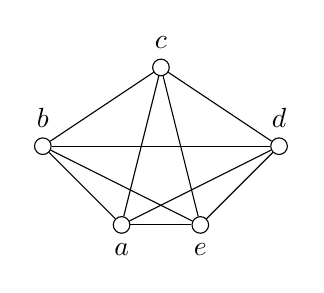
\begin{tikzpicture}
	%% the vertices
	\vertex (a) at (2,0) [label=below:$a$] {};
	\vertex (b) at (1,1) [label=above:$b$] {};
	\vertex (c) at (2.5,2) [label=above:$c$] {};
	\vertex (d) at (4,1) [label=above:$d$] {};
	\vertex (e) at (3,0) [label=below:$e$] {};			
	%% for the edges
	\path
		(a) edge (d)
		(d) edge (b)
		(b) edge (a)
		(a) edge (c)
		(b) edge (c)
		(a) edge (e)
		(e) edge (d)
		(d) edge (c)
		(c) edge (e)
		(e) edge (b)
		;
		
\end{tikzpicture}\]
\begin{center}\textit{Graph G (Figure 1.2)}\end{center}
First we have the order of $G$ defined by $|V(G)|$ is 5. Moreoever its size is 10, given by the number of edges in the graph. We can also explicitely write out the sets $V$ and $E$.
\\\\
\textbf{Definition:} We say a graph $H$ is a \textbf{subgraph} of $G$, denoted $H\subseteq G$, if we have that $V(H)\subseteq V(G)$ and $E(H) \subseteq E(G)$. If we have that $H\subseteq G$ and either $V(H)$ is a proper subset of $V(G)$ or $E(H)$ is a proper subset of $E(G)$ then we say $H$ is a \textbf{proper subgraph} of $G$.\\\\
Let us take a look at an example depicting this definition.
\[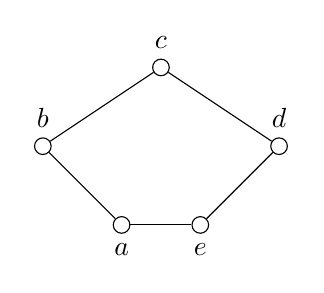
\begin{tikzpicture}
	%% the vertices for graph G
	\vertex (a) at (2,0) [label=below:$a$] {};
	\vertex (b) at (1,1) [label=above:$b$] {};
	\vertex (c) at (2.5,2) [label=above:$c$] {};
	\vertex (d) at (4,1) [label=above:$d$] {};
	\vertex (e) at (3,0) [label=below:$e$] {};			
	%% for the edges
	\path
		(a) edge (b)
		(b) edge (c)
		(c) edge (d)
		(d) edge (e)
		(e) edge (a)
		;
\end{tikzpicture}\]
\begin{center}\textit{Graph G}\end{center}
Then we have that 
\[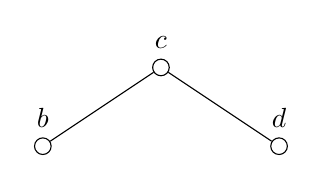
\begin{tikzpicture}
	%% the vertices for graph G
	
	\vertex (b) at (1,1) [label=above:$b$] {};
	\vertex (c) at (2.5,2) [label=above:$c$] {};
	\vertex (d) at (4,1) [label=above:$d$] {};
	%% for the edges
	\path
		(b) edge (c)
		(c) edge (d)
		
		;
\end{tikzpicture}\]
\begin{center}
\textit{Graph H}\\
\end{center}
is a subgraph of G, $H\subseteq G$\\\\
\textbf{Definition:} A subgraph $F$ of $G$ is called an \textbf{induced subgraph} of $G$ if whenever $u$ and $v$ are vertices of $F$ and $uv$ is an edge of $G$ then $uv$ is an edge of $F$.



















\end{document}
